%!TEX TS-program = PdfLaTeX
%!TEX encoding = UTF-8 Unicode


\documentclass[xcolor=x11names, compress, 11pt]{beamer}
% Options for doc
    % handout to hide navigation bar
    % compress to make slide content compressed


\mode<presentation>


%%%%%%%%%%%%%%%%%%%%%%%%%%%%%%% Define new colors %%%%%%%%%%%%%%%%%%%%%%%%%%%%%%
\definecolor{Amaranth}{rgb}{0.9, 0.17, 0.31}
\definecolor{Asparagus}{rgb}{0.53, 0.66, 0.42}
\definecolor{Amber}{rgb}{1.0, 0.49, 0.0}
\definecolor{emphase}{rgb}{0.9, 0.17, 0.31}
\definecolor{BrownGreen}{HTML}{586E75}

\definecolor{SolarizedViolet}{HTML}{6c71c4}
\definecolor{SolarizedMagenta}{HTML}{d33682}
\definecolor{SolarizedBlue}{HTML}{268bd2}
\definecolor{SolarizedCyan}{HTML}{2aa198}
\definecolor{SolarizedGreen}{HTML}{859900}
\definecolor{SolarizedRed}{HTML}{dc322f}
\definecolor{BeeYellow}{HTML}{ffcb00}
\definecolor{SolarizedOrange}{HTML}{cb4b16}
\definecolor{SolarizedYellow}{HTML}{b58900}

\definecolor{SolarizedWhite}{HTML}{fdf6e3}
\definecolor{SolarizedBrWhite}{HTML}{eee8d5}
\definecolor{GrayFrame}{HTML}{E6E6E6}
\definecolor{SolarizedBrCyan}{HTML}{93a1a1}
\definecolor{SolarizedBrBlue}{HTML}{839496}
\definecolor{SolarizedBrYellow}{HTML}{657b83}
\definecolor{SolarizedBrGreen}{HTML}{586e75}
\definecolor{SolarizedBlack}{HTML}{073642}
\definecolor{SolarizedBrBlack}{HTML}{002b36}
\definecolor{ClassicBlack}{HTML}{000000}



%%%%%%%%%%%%%%%%%%%%%%%%%%%%%%%%%%% Packages %%%%%%%%%%%%%%%%%%%%%%%%%%%%%%%%%%%
\usepackage[OT1, T1]{fontenc}                              % .pdf Encoding spec
\usepackage[utf8]{inputenc}                                % .tex Encoding spec
\usepackage[autostyle=true, threshold=0]{csquotes}         % Ensure correct quote text even nested one
\usepackage[greek, french]{babel}                          % language used
\usepackage{palatino}                                      % Font used
\usepackage{graphicx}                                      % Add images

\usepackage{hyperref}
\hypersetup{
      pdfauthor   = {Jérémy Bois},%
      pdftitle    = {Soutenance - Outil d’Aide à la Décision pour la Conception de Maisons Solaires à Énergie Positive},%
      pdfsubject  = {Soutenance Thèse - 20171009},%
}


\usepackage{color, colortbl, transparent}             % Add colors and opacity

\usepackage[separate-uncertainty=true,%
            per-mode=symbol]{siunitx}                 % Unit package
\usepackage{amsmath, amssymb, amsthm, mathtools,bm}   % Allow adding complex equations
% \usepackage{nicefrac}                               % for \nicefrac macro
% \usepackage{letltxmacro}                            % Support for optional argument in redefinition

\sisetup{output-decimal-marker={,}}                   % ... and in siunitx: dot with comma
% Writing a dot print a comma in math mode
\mathchardef\period=\mathcode`.                       % Allows to still write a dot if needed
\DeclareMathSymbol{.}{\mathord}{letters}{"3B}         % Decimal separator in math mode ...


\makeatletter % changes the catcode of @ to 11
    % Sign function
    \DeclareMathOperator{\sign}{sign}

    % Change the ways square root appears
    \let\oldr@@t\r@@t
    \def\r@@t#1#2{%
    \setbox0=\hbox{$\oldr@@t#1{#2\,}$}\dimen0=\ht0
    \advance\dimen0-0.1\ht0
    \setbox2=\hbox{\vrule height\ht0 depth -\dimen0}%
    {\box0\lower0.59pt\box2}}
    \LetLtxMacro{\oldsqrt}{\sqrt}
    \renewcommand*{\sqrt}[2][\ ]{\oldsqrt[#1]{#2}}

    % Quick and easy way to typeset abs (|) and norm (||)
    \DeclarePairedDelimiter\abs{\lvert}{\rvert}
    % Swap the definition of \abs* and \norm*, so that \abs and \norm resizes the
    % size of the brackets, and the starred version does not.
    \let\oldabs\abs
    \def\abs{\@ifstar{\oldabs}{\oldabs*}}
\makeatother % changes the catcode of @ back to 12


\usepackage{booktabs, multirow}                            % Easy pro tables and multiple row
% New columns type
\newcolumntype{B}{>{\columncolor{Amaranth}}c}
\newcolumntype{G}{>{\columncolor{Asparagus}}c}
\newcolumntype{R}{>{\columncolor{Amber}}c}


\usepackage{changepage}                                    % Enable changing text margins
\usepackage{tikz,tcolorbox}
\usepackage{cancel}



\newcommand{\hcancel}[1]{%
    \tikz[baseline=(tocancel.base)]{
        \node[inner sep=0pt,outer sep=0pt] (tocancel) {#1};
        \draw[SolarizedBrBlack] (tocancel.south west) -- (tocancel.north east);
    }%
}%



%%%%%%%%%%%%%%%%%%%%%%%%%%%%%%%%% Beamer Layout %%%%%%%%%%%%%%%%%%%%%%%%%%%%%%%%
% Head with sections
\useoutertheme[subsection=true, shadow]{miniframes}
\useinnertheme{default}
\usefonttheme{professionalfonts}
\usefonttheme{serif}

\setbeamerfont{title like}{shape=\scshape}
\setbeamerfont{frametitle}{shape=\scshape}

\setbeamercolor{bgcolor}{fg=black,bg=blue}
\setbeamercolor{section in head/foot}{bg=GrayFrame, fg=SolarizedBrBlack}
\setbeamercolor{upper separation line head}{bg=SolarizedBrWhite}
\setbeamercolor{lower separation line head}{bg=SolarizedBlue}
\setbeamercolor{middle separation line head}{bg=black!8, fg=DeepSkyBlue4}
\setbeamercolor{frametitle}{fg=SolarizedBlue,bg=SolarizedBrWhite}
\setbeamercolor{title}{fg=SolarizedBlue,bg=SolarizedBrWhite}
\setbeamercolor{normal text}{fg=ClassicBlack,bg=white}
\setbeamercolor{alerted text}{fg=SolarizedBlue,bg=SolarizedBrWhite}
\setbeamercolor{example text}{fg=ClassicBlack}
\setbeamercolor{structure}{fg=ClassicBlack}
\setbeamercolor{palette tertiary}{fg=ClassicBlack,bg=black!10}
\setbeamercolor{palette quaternary}{fg=ClassicBlack,bg=black!10}
\setbeamercolor{footlinecolor}{fg=DeepSkyBlue4,bg=black!6}

\setlength\fboxsep{0pt}
\setlength\fboxrule{0.5pt}

% Remove navigation symbols
\setbeamertemplate{navigation symbols}{}

% % Complete footline with small caps for subsection name
% \setbeamertemplate{footline}{%
%   \begin{beamercolorbox}[sep=1em,wd=\paperwidth,leftskip=0.5cm,rightskip=0.5cm]{footlinecolor}
%     \tiny
%     \hfill \textsc{\footnotesize\textbf{\author}}\hfill \insertframenumber{} / \inserttotalframenumber
%     \hfill
%   \end{beamercolorbox}%
% }


% Complete footline with small caps for subsection name
\setbeamertemplate{footline}{%
  \hfill
  \begin{beamercolorbox}[sep=0.1em, wd=0.7cm, rounded=true]{footlinecolor}
    \tiny \insertframenumber{} / \inserttotalframenumber
  \end{beamercolorbox}%
}


\defbeamertemplate*{headline}{}
{%
    % \begin{beamercolorbox}[colsep=1.5pt]{upper separation line head}
    % \end{beamercolorbox}
    \begin{beamercolorbox}[sep=0.2em]{section in head/foot}
        \vskip2pt\insertnavigation{\paperwidth}{\hfill}{\hfill}\vskip2pt
    \end{beamercolorbox}%
    \begin{beamercolorbox}[colsep=1.5pt, sep=0.2em]{middle separation line head}
        \vskip3pt \textsc{\textbf{ \footnotesize \insertsubsectionhead}} \hfill
    \end{beamercolorbox}
    \begin{beamercolorbox}[colsep=1.5pt]{lower separation line head}
    \end{beamercolorbox}
    \vskip2.5pt
}





%%%%%%%%%%%%%%%%%%%%%%%%%%%%%%%%% Specific Layout %%%%%%%%%%%%%%%%%%%%%%%%%%%%%%
\setbeamertemplate{title page}{%
  \vbox{}
  \begingroup
    \centering
    \begin{beamercolorbox}[sep=8pt,center,shadow=true,rounded=true]{title}
      \usebeamerfont{title}\inserttitle\par%
      \ifx\insertsubtitle\@empty%
      \else%
        \vskip0.25em%
        {\usebeamerfont{subtitle}\usebeamercolor[fg]{subtitle}\insertsubtitle\par}%
      \fi%
    \end{beamercolorbox}%
    \vskip1em\par
    \begin{columns}
        \begin{column}{0.3\textwidth}
            \raggedright
            \includegraphics[width=\textwidth]{Ressources/Images/Logos/bordeaux_logo.jpg}
            \vskip1em
            \includegraphics[width=\textwidth]{Ressources/Images/Logos/nouvelleAquitaine_logo.jpg}
        \end{column}
        \begin{column}{0.3\textwidth}

        \end{column}
        \begin{column}{0.3\textwidth}
            \centering
            \includegraphics[width=0.5\textwidth]{Ressources/Images/Logos/comepos_logo.png}
            \vskip1em
            \includegraphics[width=0.5\textwidth]{Ressources/Images/Logos/ademe_logo.png}
        \end{column}
    \end{columns}
    \vskip1em
    \begin{beamercolorbox}[sep=8pt,center]{author}
              \usebeamerfont{author}\insertauthor
    \end{beamercolorbox}
    \begin{beamercolorbox}[sep=8pt,center]{date}
      \usebeamerfont{date}\insertdate
    \end{beamercolorbox}
  \endgroup
}


% % Before each section
% \AtBeginSection[]
% {
%  \begin{frame}[plain]
%   \vfill
%   \centering
%   \begin{beamercolorbox}[sep=8pt,center,shadow=true,rounded=true]{title}
%     \usebeamerfont{title}\insertsectionhead\par%
%   \end{beamercolorbox}
%   \vfill
%   \end{frame}
% }




%%%%%%%%%%%%%%%%%%%%%%%%%%%%%%%%% Custom commands %%%%%%%%%%%%%%%%%%%%%%%%%%%%%%
% Add boxed subtitle
\newcommand{\addsubtitle}[1]{%
\begin{beamercolorbox}[sep=2pt,center,shadow=true,rounded=true]{footlinecolor}
    #1\par%
\end{beamercolorbox}%
}

% Add boxed alert
\newcommand{\addalert}[1]{%
\begin{beamercolorbox}[sep=2pt,center,shadow=true,rounded=true]{alerted text}
    #1\par%
\end{beamercolorbox}%
}

% Add smileys
\newcommand{\addSimley}[2]{%
\begin{tikzpicture}[scale=0.11]
    \newcommand*{\SmileyRadius}{1.5}%
    \draw [fill=#2] (0,0) circle (\SmileyRadius)% outside circle
        %node [yshift=-0.22*\SmileyRadius cm] {\tiny #1}% uncomment this to see the smile factor
        ;

    \pgfmathsetmacro{\eyeX}{0.5*\SmileyRadius*cos(30)}
    \pgfmathsetmacro{\eyeY}{0.5*\SmileyRadius*sin(30)}
    \draw [fill=SolarizedBrBlack,draw=none] (\eyeX,\eyeY) circle (0.2cm);
    \draw [fill=SolarizedBrBlack,draw=none] (-\eyeX,\eyeY) circle (0.2cm);

    \pgfmathsetmacro{\xScale}{2*\eyeX/180}
    \pgfmathsetmacro{\yScale}{1.0*\eyeY}
    \draw[color=SolarizedBrBlack, domain=-\eyeX:\eyeX]
        plot ({\x},{
            -0.1+#1*0.15 % shift the smiley as smile decreases
            -#1*1.75*\yScale*(sin((\x+\eyeX)/\xScale))-\eyeY});
\end{tikzpicture}%
}%



% \highlight[<colour>]{<stuff>}
\newcommand{\highlight}[2][SolarizedRed]{\mathchoice%
  {\colorbox{#1}{$\displaystyle#2$}}%
  {\colorbox{#1}{$\textstyle#2$}}%
  {\colorbox{#1}{$\scriptstyle#2$}}%
  {\colorbox{#1}{$\scriptscriptstyle#2$}}}%



% Add command to bubble a text with optional argument to keep same size for all
% \circled{1}       % fit argument size
% \circled{1}[10]   % fit optional argument size
\newcommand{\circled}[2][]{%
  \tikz[baseline=(char.base)]{%
    \node[shape = circle, draw, inner sep = 2pt, line width=0.5pt]
    (char) {\phantom{\ifblank{#1}{#2}{#1}}};%
    \node at (char.center) {\makebox[0pt][c]{#2}};}}
\robustify{\circled}


% Custom first page
\title{Outil d’Aide à la Décision pour la Conception de Maisons Solaires à Énergie Positive}
\author{Jérémy Bois}
\date{09/10/2017}








% % % % % % % % % % % % % % % % % % % % % % % % % % % % % % % % % % % % % % % %
\begin{document}
% % % % % % % % % % % % % % % % % % % % % % % % % % % % % % % % % % % % % % % %

\pagenumbering{Alph}
\begin{frame}[plain,noframenumbering]
\titlepage
\addtocounter{page}{-1}
\end{frame}
\pagenumbering{arabic}





% % ==============================================================================
% % ==============================================================================
\section{\scshape Contexte}
% ------------------------------------------------------------------------------
% \begin{frame}[plain]
%     \vfill
%     \centering
%     \begin{beamercolorbox}[sep=8pt,center,shadow=true,rounded=true]{title}
%     \usebeamerfont{title}\insertsectionhead\par%
%     \end{beamercolorbox}
%     \vfill
% \end{frame}


\subsection{La maison à énergie positive (MEPOS)}
\begin{frame}[t]
    \addalert{\scriptsize Production locale en énergie renouvelable $>$ Consommation}
    \vfill
    \centering
    \begin{columns}
        \begin{column}{0.45\textwidth}
            \centering
            \uncover<2->{%
            Bilan
            \begin{itemize}
                \scriptsize
                \item Énergie \uncover<3->{finale / primaire}
                \item<3-> $CO_{2}$
                \item<3-> Économique
            \end{itemize}
            }
            \vskip3.5em
            \uncover<5->{%
            \begin{itemize}
                \scriptsize
                \item 5 usages
                \item Adéquation temporelle
            \end{itemize}
            }
        \end{column}%
        \begin{column}{0.7\textwidth}
            \centering
            \uncover<2->{%
            \includegraphics[height=0.5\textheight]{Ressources/Images/Soutenance/Contexte_objectifs/bilan_nzeb_fr.pdf}
            }
            \vskip1.25em
            \uncover<4->{%
            \includegraphics[height=0.25\textheight]{Ressources/Images/Soutenance/Contexte_objectifs/hurdle_race.pdf}
            }
        \end{column}%
    \end{columns}%

            \note{À faire en français}
\end{frame}



% ------------------------------------------------------------------------------
\subsection{L’énergie solaire}
\begin{frame}[c]
    \vfill
    \centering
    \small
    \includegraphics[height=0.6\textheight]{Ressources/Images/Environnement/evolution_enr.png}
    \begin{columns}
        \begin{column}{0.45\textwidth}
            \begin{center}
                \begin{itemize}
                    \item Progression forte du photovoltaïque
                \end{itemize}
            \end{center}
        \end{column}%
        \begin{column}{0.45\textwidth}
            \begin{center}
            \begin{itemize}
                \item Progression solaire thermique lente
            \end{itemize}
            \end{center}
        \end{column}%
    \end{columns}%
    \vfill
    \uncover<2->{%
    \addalert{Moyenne en France~: \SI{1112}{kWh\per\metre\squared\per an}}
    }
    % http://www.travaux.com/dossier/construction-ecologique/12274/Baisse-des-tarifs-d-achat-du-photovoltaique-pour-2011.html
    % http://www.lefigaro.fr/impots/2010/09/06/05003-20100906ARTFIG00493-les-aides-au-photovoltaique-reduites-de-moitie.php
    % Chute du crédit d'impôt photovoltaïque en 2011 50 à 25\% + baisse du tarif de rachat 58 à 46 expliquant la chute de progression.
\end{frame}


% ------------------------------------------------------------------------------
\subsection{Les systèmes solaires combinés}
\begin{frame}[c]
    \vfill
    \centering
    \small
    \includegraphics[width=\textwidth]{Ressources/Images/Soutenance/Contexte_objectifs/energie_icones.png}
    \vfill
    \uncover<2->{%
    \begin{columns}
        \begin{column}{0.45\textwidth}
            \begin{center}
                \begin{itemize}
                    \item SSC sur le marché Européen
                \end{itemize}
            \end{center}
        \end{column}%
        \begin{column}{0.45\textwidth}
            \begin{center}

                \begin{itemize}
                    \item Majoritairement en maison individuelle
                \end{itemize}
            \end{center}
        \end{column}%
    \end{columns}%
    }
    \vfill
    \uncover<3->{\addalert{BEPOS avec SSC $< \SI{10}{\percent}$}}
    \vfill
\end{frame}



% ------------------------------------------------------------------------------
\subsection{Sommaire}
\begin{frame}[t]
\raggedright
\vfill
Description de la problématique
\vfill
Présentation de la méthodologie d’optimisation développée.
\vfill
Application au dimensionnement d’une MEPOS solaire.
\vfill
Conclusions et perspectives.
\vfill
\end{frame}


















% % ==============================================================================
% % ==============================================================================
\section{\scshape Problématique}
% ------------------------------------------------------------------------------
\subsection{Description du problème}
\begin{frame}[c]
    \vfill
    \only<1>{\includegraphics[width=0.95\textwidth]{Ressources/Images/Soutenance/Problematique/modele_generique_base.pdf}}
    \only<2>{\includegraphics[width=0.95\textwidth]{Ressources/Images/Soutenance/Problematique/modele_generique_ECS.pdf}}
    \only<3>{\includegraphics[width=0.95\textwidth]{Ressources/Images/Soutenance/Problematique/modele_generique_besoinsCH.pdf}}
    \only<4>{\includegraphics[width=0.95\textwidth]{Ressources/Images/Soutenance/Problematique/modele_generique_CH.pdf}}
    \only<5>{\includegraphics[width=0.95\textwidth]{Ressources/Images/Soutenance/Problematique/modele_generique_final.pdf}}
    \vfill
\end{frame}



% ------------------------------------------------------------------------------
\subsection{Combinatoire du problème}
\begin{frame}[c]
    \vfill
    \centering
    \begin{columns}
        \begin{column}{0.4\textwidth}
            \vskip1em
            \addsubtitle{Nombreux facteurs}
            \vskip6.5em
            \uncover<2->{%
            \addsubtitle{Forte hétérogénéité}
            }
        \end{column}
        \begin{column}{0.65\textwidth}
            \begin{itemize}
                \item Scénario d’usages
                \item Équipements du SSC
                \item Logique de contrôle associée
                \item Production photovoltaïque
                \item Enveloppe du bâtiment
            \end{itemize}
            \vskip2em
            \uncover<2->{%
            \begin{itemize}
                \item continus
                \item discrets
                \item qualitatifs
            \end{itemize}
            }
        \end{column}
    \end{columns}
    \vskip0.5em
    \vfill
    \uncover<3->{\addalert{Combinatoire importante}}
\end{frame}


% ------------------------------------------------------------------------------
\subsection{Objectifs / Contraintes}
\begin{frame}[t]
    % \addalert{\usebeamerfont{frametitle} \footnotesize \textbf{Objectif~: valoriser l’énergie solaire pour des MEPOS}}
    \vfill
    \begin{adjustwidth}{-2em}{-2em}
        \begin{beamercolorbox}[sep=1pt, wd=2.5cm, center,shadow=true,rounded=true]{footlinecolor}
             Objectifs\par%
        \end{beamercolorbox}
        \vskip0.5em
        \begin{itemize}
            \small
            \item Évaluer la performance du SSC pour une MEPOS.
            \vskip1em
            \item Optimiser l’adéquation entre besoins / production / consommations.
        \end{itemize}

        \vskip3em

        \uncover<2->{
            \begin{beamercolorbox}[sep=1pt, wd=2.5cm, center,shadow=true,rounded=true]{footlinecolor}
                 Contraintes\par%
            \end{beamercolorbox}
        }
        \vskip0.5em

        \begin{itemize}
            \small
            \item<2-> Problématique multi-critères et multi-physiques. \\
            \vskip1em
            \item<2-> Partager la surface disponible en toiture.
        \end{itemize}
        \vfill
    \end{adjustwidth}
\end{frame}





% ------------------------------------------------------------------------------
\subsection{Formulation du problème}
\begin{frame}[t]
    \footnotesize
    \vfill
    \begin{adjustwidth}{-2em}{-2em}
        \begin{columns}
            \begin{column}{0.6\textwidth}
                \includegraphics[width=1.15\textwidth]{Ressources/Images/Soutenance/Problematique/modele_generique_eq.pdf}
            \end{column}
            \begin{column}{0.4\textwidth}
                \vskip3em
                \begin{subequations}
                        \begin{align*}
                            Conso_{ECS} &= Conso^{ECS}_{app} +  Prod^{ECS}_{sol} \\
                            Conso_{CH} &= Conso^{CH}_{app} +  Prod^{CH}_{sol}
                        \end{align*}
                \end{subequations}
                \uncover<2->{
                \begin{subequations}
                    \begin{align*}
                        Conso_{usages} &= Conso_{Electromenager} \\
                                       &\quad + Conso_{Eclairage}
                    \end{align*}
                \end{subequations}
                }
            \end{column}
        \end{columns}
        \vskip1em
        \uncover<3->{%
        \begin{equation*}
            Prod_{PV}  + Prod^{CH}_{sol} + Prod^{ECS}_{sol} - Conso_{usages} - Conso_{ECS} - Conso_{CH} \geq 0
        \end{equation*}
        }
        \vfill
        \uncover<4->{%
        \addalert{\normalsize $Prod_{PV} - Conso_{usages} - Conso_{app} \geq 0$}
        }
    \end{adjustwidth}
    \vfill
\end{frame}



\begin{frame}[t]
    \addalert{$Prod_{PV} - Conso_{usages} - Conso_{app} \geq 0$}
    \vfill
    \small
    \begin{columns}
        \begin{column}{0.2\textwidth}
            \vskip3.5em
            \uncover<4->{\addsubtitle{Objectifs}}
            \vskip7em
            \uncover<6->{\addsubtitle{Contraintes}}
        \end{column}%
        \begin{column}{0.8\textwidth}
                \begin{itemize}
                    \item \only<1-3>{Évaluer la performance du SSC} \only<4->{Maximiser la performance du SSC}
                \end{itemize}
                \begin{columns}
                    \begin{column}{0.5\textwidth}
                        \centering
                        \only<1-2>{$F_{sol}       = \frac{Prod_{sol}}{Prod_{sol} + Conso_{app}}$}
                        \only<3>{{\color{SolarizedRed} \cancel{$F_{sol}       = \frac{Prod_{sol}}{Prod_{sol} + Conso_{app}}$}}}
                        \only<4->{$F_{sav}^{CH}   = 1 - \frac{Conso_{app}^{CH}}{Conso_{ref}^{CH}}$}
                    \end{column}
                    \begin{column}{0.5\textwidth}
                        \centering
                        \only<2>{$F_{sav}  = 1 - \frac{Conso_{app}}{Conso_{ref}}$}
                        \only<3>{{\color{SolarizedGreen} $F_{sav}  = 1 - \frac{Conso_{app}}{Conso_{ref}}$}}
                        \only<4->{$F_{sav}^{ECS}   = 1 - \frac{Conso_{app}^{ECS}}{Conso_{ref}^{ECS}}$}
                    \end{column}
                \end{columns}
            \vskip0.5em
            % \only<4>{\includegraphics[height=0.6\textheight]{Ressources/Images/Modelisation/Principe/air_elec_mono.pdf}}
            \begin{itemize}
                \item<5-> Maximiser la production des capteurs PV.
                \item<5-> Minimiser la surface de capteurs PV.
            \end{itemize}
            \vskip2em
            \uncover<6->{%
                \begin{itemize}
                    \item Partage de la surface disponible en toiture.
                    \item<7-> \footnotesize $\abs{Prod_{PV} - Conso_{usages} - Conso_{app}}  \geq  8 \si{kWh_{ep}\per\metre\squared\per an}$
                \end{itemize}
            }
        \end{column}
    \end{columns}
    \vfill
\end{frame}



% ------------------------------------------------------------------------------
\subsection{Verrous à lever}
\begin{frame}[t]
    \vfill
    \small
    \begin{itemize}
        \item Capacité à mettre en œuvre la modélisation complexe nécessaire.
        \vfill
        \item Sélectionner une méthodologie d’optimisation adaptée.
        \begin{itemize}
            \footnotesize
            \item[--] afin de tenir compte de plusieurs objectifs.
            \vskip0.5em
            \item[--] afin de converger vers un ensemble de solutions optimales.
        \end{itemize}
        \vfill
        \item Accompagner le décideur dans son choix.
    \end{itemize}
    \vfill
\end{frame}




% % ==============================================================================
% % ==============================================================================
\section{\scshape Méthode d’optimisation}
% ------------------------------------------------------------------------------
\begin{frame}[plain]
    \vfill
    \centering
    \begin{beamercolorbox}[sep=8pt,center,shadow=true,rounded=true]{title}
    \usebeamerfont{title}Méthode d’optimisation développée\par%
    \end{beamercolorbox}
    \vfill
\end{frame}


\subsection{Optimisation et décision}
\begin{frame}[t]
    \addsubtitle{La décision précède l’optimisation}
    \vfill
    \centering
    \only<1>{\includegraphics[width=0.8\textwidth]{Ressources/Images/Soutenance/Methodologie/decision_a_priori.pdf}}
    \only<2>{\includegraphics[width=0.8\textwidth]{Ressources/Images/Soutenance/Methodologie/decision_a_priori_detail.pdf}}
    \vfill
\end{frame}


\begin{frame}[t]
    \addsubtitle{L’optimisation précède la décision}
    \vfill
    \centering
    \begin{adjustwidth}{-2.1em}{-2.1em}
     \begin{columns}
        \begin{column}{0.42\textwidth}
            \raggedright
            \begin{itemize}
                \item<2-> Variables hétérogènes
                \vskip-0.5em
                \begin{itemize}
                    \item<2->[--] Qualitatives
                    \item<2->[--] Discrètes
                    \item<2->[--] Continues
                \end{itemize}
                \vskip0.5em
                \item<3-> Combinatoire importante
                \vskip0.5em
                \item<4-> Connaissance limitée
            \end{itemize}
        \end{column}%
        \begin{column}{0.74\textwidth}
            \centering
            \only<1>{\includegraphics[width=\textwidth]{Ressources/Images/Soutenance/Methodologie/decision_a_posteriori.pdf}}
            \only<2>{\includegraphics[width=\textwidth]{Ressources/Images/Soutenance/Methodologie/decision_a_posteriori_type.pdf}}
            \only<3>{\includegraphics[width=\textwidth]{Ressources/Images/Soutenance/Methodologie/decision_a_posteriori_cardinalite.pdf}}
            \only<4->{\includegraphics[width=\textwidth]{Ressources/Images/Soutenance/Methodologie/decision_a_posteriori_meta.pdf}}
        \end{column}%
    \end{columns}%
    \end{adjustwidth}
    \vfill
    \uncover<5>{\addalert{Comment classer des solutions ayant plusieurs objectifs~?}}
    \vfill
\end{frame}

\begin{frame}[t]
    \addsubtitle{Dominance au sens de Pareto}
    \vfill
    \centering
    \begin{columns}
        \begin{column}{0.45\textwidth}
            \centering
            \small
            \uncover<2->{%
            Relation de dominance \\ \vskip1em
            + \\  \vskip1em
            Ensemble de solutions \\  \vskip2em
            = \\  \vskip2em
            Front de Pareto
            }
        \end{column}%
        \begin{column}{0.7\textwidth}
            \centering
            \only<1>{\includegraphics[width=0.98\textwidth]{Ressources/Images/Soutenance/Methodologie/dominance_0.pdf}}
            \only<2->{\includegraphics[width=0.98\textwidth]{Ressources/Images/Soutenance/Methodologie/dominance_1.pdf}}
        \end{column}%
    \end{columns}%
    \vfill
    \uncover<3>{\addalert{Quel algorithme d’optimisation choisir~?}}
\end{frame}



% ------------------------------------------------------------------------------
\subsection{Optimisation par Colonie d’Abeilles Virtuelles}
\begin{frame}[t]
    \addalert{\footnotesize Exploration~: $NP$ \hfill Exploitation~: $Max_{echec}$}
    \vskip0.25em
    \centering
    \only<2>{\includegraphics[height=0.95\textheight]{Ressources/Images/Soutenance/Methodologie/comportement_abeilles_steps_1.pdf}}
    \only<3>{\includegraphics[height=0.95\textheight]{Ressources/Images/Soutenance/Methodologie/comportement_abeilles_steps_2.pdf}}
    \only<4>{\includegraphics[height=0.95\textheight]{Ressources/Images/Soutenance/Methodologie/comportement_abeilles_steps_3.pdf}}
    \only<5>{\includegraphics[height=0.95\textheight]{Ressources/Images/Soutenance/Methodologie/comportement_abeilles_steps_4.pdf}}
    \only<6>{\includegraphics[height=0.95\textheight]{Ressources/Images/Soutenance/Methodologie/comportement_abeilles_steps_5.pdf}}
    \vfill
\end{frame}


\begin{frame}[c]
    \vfill
    \centering
    \begin{adjustwidth}{-2.2em}{-2em}
    \begin{columns}
        \begin{column}{0.4\textwidth}
            \raggedright
            \footnotesize

            % Initialisation
            \uncover<2->{%
            \textbf{Initialisation}\\
            \vskip0.4em
            \includegraphics[width=1.1\textwidth]{Ressources/Images/Soutenance/Methodologie/principe_obl.pdf}
            \vskip2em
            }

            % Maj butineuses
            \uncover<3->{%
            \textbf{Butineuses}\\
            \vskip0.3em
            \begin{itemize}
                \item Exploration
                \item Mouvement uniforme
                \item \alt<6->{\colorbox{SolarizedRed!70}{Vol de Lévy}}{Vol de Lévy}
            \end{itemize}
            \vskip2em
            }

            % Maj ouvrières
            \uncover<4->{%
            \textbf{Ouvrières} \\
            \begin{itemize}
                \item Exploitation
                \item Mouvement uniforme
            \end{itemize}
            \vskip2em
            }

            \uncover<5->{%
            \textbf{Exploratrices}
            \begin{itemize}
                \item Position réinitialisée
            \end{itemize}
            }

        \end{column}%
        \begin{column}{0.6\textwidth}
            \raggedright
            \vskip0.5em
            \begin{tikzpicture}
                \node[anchor=south west,inner sep=0] (image) at (0,0) {\includegraphics[width=1.05\textwidth]{Ressources/Images/Soutenance/Methodologie/algorithme_complet.pdf}};
                \begin{scope}[x={(image.south east)},y={(image.north west)}]
                    \draw<6-> [SolarizedRed,ultra thick,rounded corners] (0,0.4) rectangle (0.35,0.7);
                \end{scope}
            \end{tikzpicture}

        \end{column}%
    \end{columns}%
    \end{adjustwidth}
    \vfill
\end{frame}


\begin{frame}[t]
    \addsubtitle{Mise à jour~: $\epsilon$-Archive}
    \vfill
    \centering
    \includegraphics[height=0.8\textheight]{Ressources/Images/Soutenance/Methodologie/selection_boxes.pdf}
    \vfill
\end{frame}


\begin{frame}[t]
    \addsubtitle{Vol de Lévy}
    \vfill
    \centering
    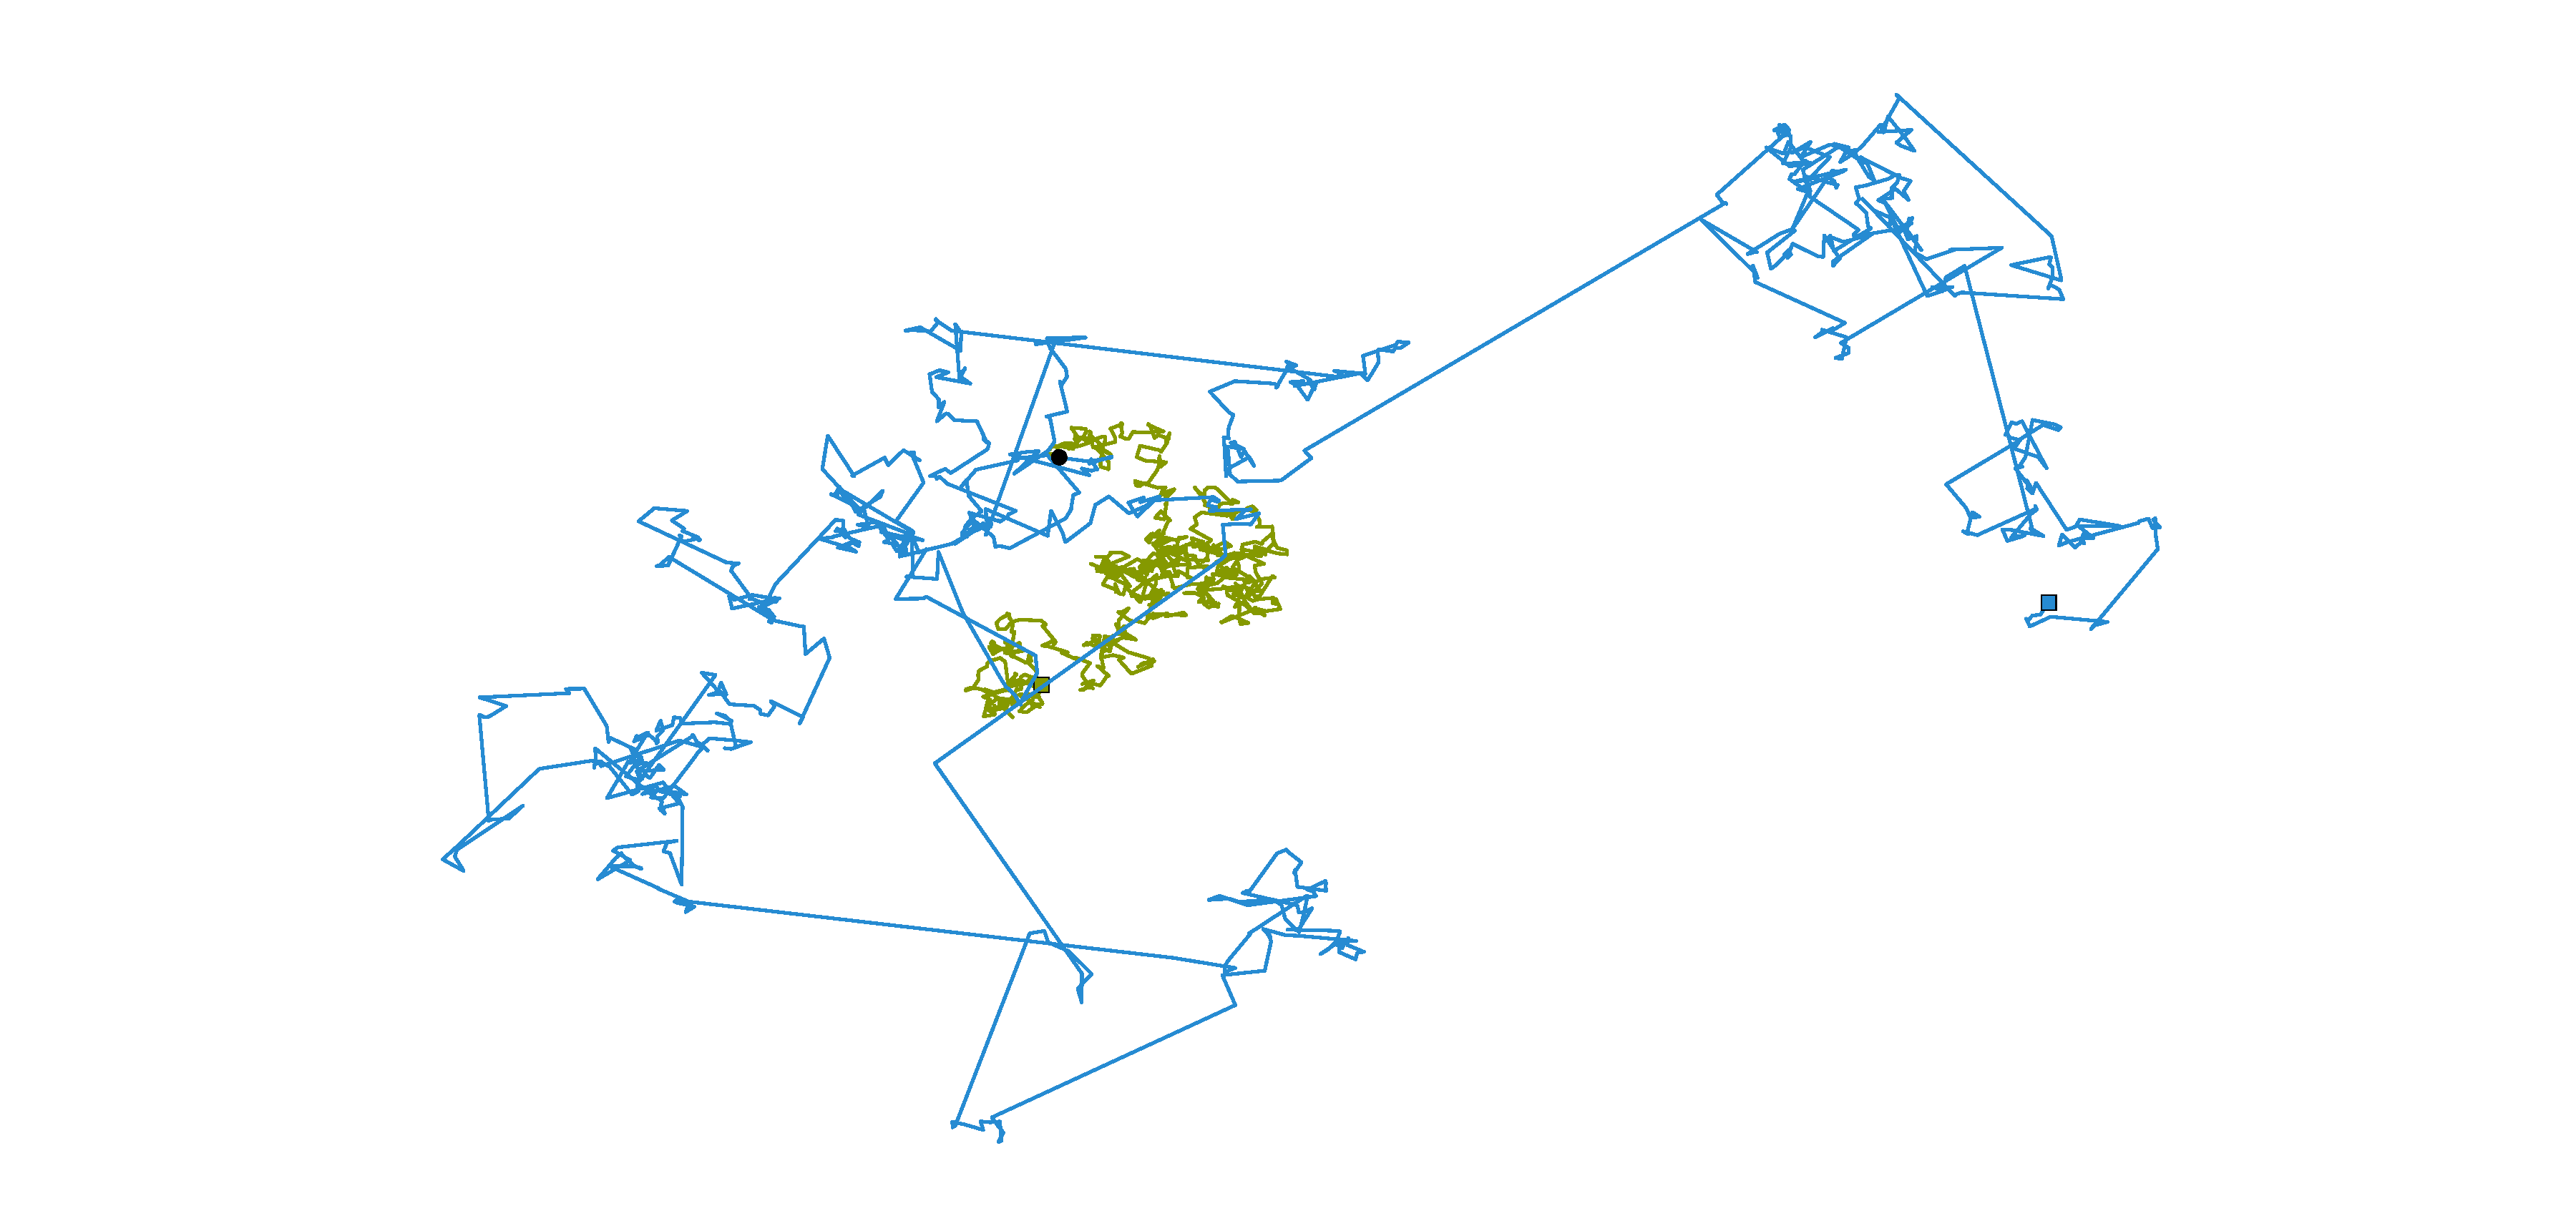
\includegraphics[height=0.8\textheight, clip=true, trim=100mm 10mm 90mm 10mm]{Ressources/Images/Optimisation/LevyFlight/levy_vs_gaussian.pdf}
    \vfill
\end{frame}



% ------------------------------------------------------------------------------
\subsection{Réduction de la cardinalité}
\begin{frame}[t]
    \vfill
    \centering
    \small
    \begin{columns}
        \begin{column}{0.4\textwidth}
            \vskip1em
            \addsubtitle{Systèmes solaires}
            \vskip6em
            \uncover<2->{%
            \addsubtitle{Bâtiment}
            }
        \end{column}
        \begin{column}{0.65\textwidth}
            \begin{itemize}
                \item Nombre de capteurs
                \item Isolation des ballons
                \item \dots
            \end{itemize}
            \vskip2em
            \uncover<2->{%
            \begin{itemize}
                \item Résistance thermique du plancher
                \item Surface de vitrage
                \item \dots
            \end{itemize}
            }
        \end{column}
    \end{columns}
    \vskip0.5em
    \vfill
    \uncover<3->{\addalert{Quels sont les paramètres les plus influents~?}}
\end{frame}



\begin{frame}[t]
    \addsubtitle{Criblage de Morris}
    \vfill
    \centering
    \small
    \begin{columns}
        \begin{column}{0.4\textwidth}
        \centering
        \uncover<2->{%
        \circled[3]{1} Définition des bornes\\
        \includegraphics[height=0.35\textheight]{Ressources/Images/Soutenance/Methodologie/morris_definition.pdf}
        }
        \vskip1.5em
            \uncover<4->{%
            \circled[3]{3} Évaluation de l’influence\\
            \includegraphics[height=0.3\textheight]{Ressources/Images/Soutenance/Methodologie/morris_analyse.pdf}
            }
        \end{column}%
        \begin{column}{0.7\textwidth}
            \centering
            \uncover<3->{%
            \circled[3]{2} Création d’un plan d’expérience\\
            \includegraphics[height=0.6\textheight]{Ressources/Images/Soutenance/Methodologie/cube_morris_axes.pdf}
            }
        \end{column}%
    \end{columns}%
    \vfill
\end{frame}











% % ==============================================================================
% % ==============================================================================
\section{\scshape Application}
% ------------------------------------------------------------------------------
\begin{frame}[plain]
    \vfill
    \centering
    \begin{beamercolorbox}[sep=8pt,center,shadow=true,rounded=true]{title}
    \usebeamerfont{title}Application au dimensionnement d’une MEPOS solaire\par%
    \end{beamercolorbox}
    \vfill
\end{frame}

% ------------------------------------------------------------------------------
\subsection{Conditions limites de l’étude}
\begin{frame}[t]
    \centering
    \addalert{\small Deux climats étudiés~: \textbf{Bordeaux} et \textbf{Strasbourg}}
    \vfill
    \scriptsize
    \begin{columns}
        \begin{column}{0.5\textwidth}
            \vskip0.5em
            \includegraphics[width=\textwidth]{Ressources/Images/Soutenance/CasEtude/maison_photo.jpg}
            \vskip0.25em
            \begin{table}
                \begin{tabular}{l c c c}
                    \toprule
                                                   & Bordeaux           &  & Strasbourg          \\
                    \midrule
                    $DJU$ (\SI{19}{\celsius})      & \num{2408}         &  & \num{3360}          \\
                    \addlinespace[\defaultaddspace]
                    $T_{EF}$ (\si{\celsius})       & \num{8.9} à \num{16}  &  & \num{5.3} à \num{14}    \\
                    \bottomrule
                \end{tabular}
                \end{table}
        \end{column}
        \begin{column}{0.5\textwidth}
            \uncover<2->{\includegraphics[height=0.75\textheight, clip=true, trim=200mm 0mm 0mm 0mm]{Ressources/Images/EtudeDeCas/irradiations_climats.pdf}}
        \end{column}
    \end{columns}
    \vfill
\end{frame}


% ------------------------------------------------------------------------------
\subsection{Hypothèses}
\begin{frame}[c]
    \vfill
    \centering
    \begin{columns}
        \begin{column}{0.4\textwidth}
            \addsubtitle{Charges internes}~\\[0.5em]
            Inoccupation~: \SI{16}{\celsius}\\[0.5em]
            Occupation (jour)~: \SI{19}{\celsius}\\[0.5em]
            Occupation (nuit)~: \SI{18}{\celsius}
            \vskip3.5em
            \uncover<2->{%
            \addsubtitle{Puisage~: \SI{33}{l\per (jour\period pers)}}~\\
            Pondération~:
            \begin{itemize}
                \item journalière
                \item mensuelle
            \end{itemize}
            }
        \end{column}
        \begin{column}{0.7\textwidth}
            \raggedleft
            \vskip1em
            \includegraphics[width=0.9\textwidth]{Ressources/Images/Modelisation/Scenario/charges_internes.pdf}
            \vskip2em
            \uncover<2->{\includegraphics[width=0.9\textwidth]{Ressources/Images/Soutenance/CasEtude/puisage_realiste.pdf}}
        \end{column}
    \end{columns}
    \vfill
\end{frame}


\subsection{Système étudié}
\begin{frame}[c]
    \vfill
    \centering
    \includegraphics[width=\textwidth]{Ressources/Images/Soutenance/Application/air_complet_mono_PV.pdf}
    \vfill
\end{frame}

\subsection{Système de référence}
\begin{frame}[c]
    \vfill
    \centering
    \includegraphics[width=0.85\textwidth]{Ressources/Images/Soutenance/Application/air_complet_ref.pdf}
    \vfill
\end{frame}


% ------------------------------------------------------------------------------
\subsection{Outil de Modélisation}
\begin{frame}[t]
    \vfill
    \centering
    \includegraphics[width=0.6\textwidth, clip=true, trim=0mm 228mm 0mm 0mm]{Ressources/Images/chapitre3_bilan.pdf}
    \vfill
\end{frame}


\begin{frame}[t]
    \centering
    \begin{columns}
        \begin{column}{0.45\textwidth}
            \centering
            \addsubtitle{Langage / Logiciel}
            \begin{itemize}
                \item Multi-physiques
                \item Équationnel
                \item Acausal
            \end{itemize}
            \vskip1em
            \includegraphics[width=0.5\textwidth]{Ressources/Images/Logos/modelica_logo.png}
            \includegraphics[width=0.5\textwidth]{Ressources/Images/Logos/dymola_logo.jpg}
        \end{column}%
        \begin{column}{0.55\textwidth}
            \centering
            \uncover<2->{%
            \addsubtitle{Bibliothèque}
            \begin{itemize}
                \item Activement maintenue
                \item Large choix de composants
                \item Libre et ouverte
            \end{itemize}
            \vskip1em
            \includegraphics[width=0.4\textwidth]{Ressources/Images/Logos/Buildings_logo.png}
            }
        \end{column}%
    \end{columns}%
\end{frame}

% ------------------------------------------------------------------------------
\subsection{Réduction de la complexité}
\begin{frame}[t]
    \begin{adjustwidth}{-2em}{-2em}
        \only<1>{\includegraphics[height=0.8\textheight, clip=true trim0mm 0mm 0mm 2mm]{Ressources/Images/Soutenance/Application/SSC_capture.png}}
        \only<2->{\includegraphics[height=0.8\textheight, clip=true trim0mm 0mm 0mm 2mm]{Ressources/Images/Soutenance/Application/SSC_capture_work.png}}
    \end{adjustwidth}
    \vfill
    \uncover<3->{%
    \begin{columns}
        \begin{column}{0.5\textwidth}
            \addalert{\small $> \num{22500}$ équations}
        \end{column}
        \begin{column}{0.5\textwidth}
            \addalert{\small Simulation $\sim$ \num{1} à \SI{3}{h}}
        \end{column}
    \end{columns}
    }
\end{frame}

\begin{frame}[t]
    \addsubtitle{Méta-modèles par chaos polynomial}
    \vfill
    \centering
    \textbf{Approximation des objectifs par des fonctions analytiques}
    \uncover<2->{%
    \begin{columns}
        \begin{column}{0.5\textwidth}
            \begin{itemize}
                \item $Conso_{app}$
                \item $Conso_{app}^{CH}$
            \end{itemize}
        \end{column}
        \begin{column}{0.5\textwidth}
            \begin{itemize}
                \item $Conso_{app}^{ECS}$
                \item $Conso_{ref}^{CH}$
            \end{itemize}
        \end{column}
    \end{columns}
    }
    \vskip2em
    \begin{columns}
        \begin{column}{0.5\textwidth}
            \centering
            \uncover<3->{%
            \circled[3]{1} Définition d’un échantillon représentatif
            \includegraphics[width=1\textwidth]{Ressources/Images/MetaModele/halton_vs_uniform.pdf}
            }
        \end{column}
        \begin{column}{0.6\textwidth}
            \centering
            \uncover<4->{%
            \circled[3]{2} Minimisation de l’erreur quadratique moyenne \\
            \raggedright
            \begin{equation*}
                \highlight[SolarizedRed!70]{\min(f(\vec{x}) - \mathcal{M}(\vec{x}))}
            \end{equation*}
            \vskip0.5em
            \begin{equation*}
                \mathcal{M}(\vec{x}) \approx \sum c_{\vec{\alpha}} \times \psi_{\vec{\alpha}}(\,\underline{\vec{x}}\,)
                % \mathcal{M}(\vec{x}) \approx \sum_{\abs{\vec{\alpha}} \leq P} c_{\vec{\alpha}} \times \psi_{\vec{\alpha}}(\,\underline{\vec{x}}\,)
            \end{equation*}
            }
        \end{column}
    \end{columns}
    \vfill
\end{frame}




% ------------------------------------------------------------------------------
\subsection{Réduction de la cardinalité}
\begin{frame}[t]
    \vfill
    \centering
    \includegraphics[width=0.6\textwidth, clip=true, trim=0mm 178mm 0mm 0mm]{Ressources/Images/chapitre3_bilan.pdf}
    \vfill
\end{frame}

\begin{frame}[t]
    \vfill
    \centering
    \begin{columns}
        \begin{column}{0.75\textwidth}
            \uncover<2->{%
                \includegraphics[height=0.9\textheight]{Ressources/Images/Soutenance/Application/graphInfluence.pdf}
            }
        \end{column}
        \begin{column}{0.3\textwidth}
            \centering
            \tiny
            \addsubtitle{\footnotesize 21 facteurs a priori}
            \vskip3em
            \uncover<3->{%
            \addsubtitle{\footnotesize Bordeaux~: 14}
            \hbox{\cancel{Surface vitrée Sud / Nord / Ouest}}
            \hbox{\cancel{Résistance thermique plancher}}
            \hbox{\cancel{Isolation ballon sanitaire}}
            \hbox{\cancel{Isolation canalisation}}
            \hbox{\cancel{Consigne algorithme~: $T3_{min}$}}
            \vskip3em
            \addsubtitle{\footnotesize Strasbourg~: 15}
            \hbox{\cancel{Surface vitrée Nord / Ouest}}
            \hbox{\cancel{Isolation ballon stockage et sanitaire}}
            \hbox{\cancel{Isolation canalisation}}
            \hbox{\cancel{Consigne algorithme~: $T3_{min}$}}
            }
        \end{column}
    \end{columns}
    \vfill
\end{frame}




% ------------------------------------------------------------------------------
\subsection{Création des méta-modèles}
\begin{frame}[t]
    \vfill
    \centering
    \includegraphics[width=0.6\textwidth, clip=true, trim=0mm 128mm 0mm 0mm]{Ressources/Images/chapitre3_bilan.pdf}
    \vfill
\end{frame}

\begin{frame}[c]
    \centering
    \tiny
    \begin{table}
    Erreurs relatives (\si{\percent}) | RMSE = Erreur quadratique moyenne | MAE = Erreur absolue maximale
    \vskip0.4em
    \begin{tabular}{l c c c c c c}
        \toprule
                        & \multicolumn{2}{c}{Bordeaux} & & \multicolumn{2}{c}{Strasbourg} &
                          Taille \\
                        \cmidrule(r){2-3}
                        \cmidrule(r){5-6}
                        & $RMSE$ & $MAE$   &       & $RMSE$ & $MAE$ & échantillon \\
        \midrule
        $Conso_{ref}^{CH}$  & \alt<1>{\cellcolor{SolarizedGreen}}{}\num{0.05}  & \alt<1>{\cellcolor{SolarizedGreen}}{}\num{0.1}  &  & \num{0.01}   & \num{0.03}  & \alt<1>{\cellcolor{SolarizedGreen}}{}\num{400}  \\
        \addlinespace[\defaultaddspace]
        $Conso_{app}^{CH}$  & \alt<2>{\cellcolor{SolarizedRed}}{}\num{3.5}  & \num{6.5} &  & \num{1.3}   & \num{2.6}  & \alt<2>{\cellcolor{SolarizedGreen}}{}\num{600} \\
        \addlinespace[\defaultaddspace]
        $Conso_{app}^{ECS}$ & \num{3.0} & \alt<2>{\cellcolor{SolarizedRed}}{}\num{8.1} & & \num{2.7}   & \num{6.8}  & \alt<2>{\cellcolor{SolarizedGreen}}{}\num{600} \\
        \addlinespace[\defaultaddspace]
        $Conso_{app}$       & \num{2.2} & \num{5.6} & & \num{1.0}   & \num{2.7}  & \alt<2>{\cellcolor{SolarizedGreen}}{}\num{600} \\
        \bottomrule
    \end{tabular}
    \end{table}
    \vskip0.5em
    \uncover<3->{\includegraphics[width=0.9\textwidth, clip=true, trim=0mm 100mm 0mm 0mm]{Ressources/Images/MetaModele/validite_meta_ssc_600.pdf}}
\end{frame}



% ------------------------------------------------------------------------------
\subsection{Optimisation multi-objectifs}
\begin{frame}[t]
    \vfill
    \centering
    \includegraphics[width=0.6\textwidth, clip=true, trim=0mm 77mm 0mm 0mm]{Ressources/Images/chapitre3_bilan.pdf}
    \vfill
\end{frame}



% ------------------------------------------------------------------------------
\subsection{Optimisation multi-objectifs~: Potentiel du SSC}
\begin{frame}[c]
    \vfill
    \centering
    \scriptsize
    \begin{table}
    \centering
    % Variation de la performance pour les solutions optimales.
    % \vskip1.5em
    \begin{tabular}{l c c c c c c c c}
        \toprule
                        & & & \multicolumn{2}{c}{Bordeaux} & & & \multicolumn{2}{c}{Strasbourg} \\
                        \cmidrule(r){4-5}
                        \cmidrule(r){8-9}
                        & & & min & max   &       & & min & max \\
        \midrule
        \multirow{3}{*}{Référence (\si{kWh})} & ECS & &  \multicolumn{2}{c}{\alt<1>{\cellcolor{SolarizedBrWhite}}{}2588}  & &  & \multicolumn{2}{c}{\alt<1>{\cellcolor{SolarizedBrWhite}}{}2866}  \\
        \addlinespace[\defaultaddspace]
                                   & CH  & &  \alt<3>{\cellcolor{SolarizedRed}}{} \num{228}  & \alt<2>{\cellcolor{SolarizedRed}}{}\num{620} & &  & \alt<3>{\cellcolor{SolarizedGreen}}{} \num{1363}   & \alt<2>{\cellcolor{SolarizedGreen}}{} \num{2110} \\
        \addlinespace[\defaultaddspace]
                                   & ECS + CH & & \alt<4>{\cellcolor{SolarizedRed}}{} \num{2816} & \num{3208} & & & \alt<4>{\cellcolor{SolarizedGreen}}{}\num{4229}   & \num{4976} \\
        \\
        \addlinespace[\defaultaddspace]
        \uncover<5->{Appoint (\si{\percent})  & $F_{sav,\,ext}$ & &  \num{57} & \uncover<5->{\cellcolor{SolarizedGreen}}{}\num{90} & & & \num{42}   & \uncover<5->{\cellcolor{SolarizedGreen}}{}\num{72}} \\
        \\
        \addlinespace[\defaultaddspace]
        \uncover<6->{Appoint (\si{kWh}) & ECS + CH & &  \alt<6>{\cellcolor{SolarizedRed}}{} \num{324} & \alt<6>{\cellcolor{SolarizedRed}}{} \num{1372} & & & \alt<6>{\cellcolor{SolarizedGreen}}{} \num{1222}   & \alt<6>{\cellcolor{SolarizedGreen}}{} \num{3117}} \\
        \bottomrule
    \end{tabular}
    \end{table}
    \vfill
\end{frame}


% ------------------------------------------------------------------------------
\subsection{Optimisation multi-objectifs~: Diversité des solutions}
\begin{frame}[t]
    % \addsubtitle{Résultats d’optimisation sur Strasbourg}
    % \vskip1em
    \begin{adjustwidth}{-2.4em}{-2.4em}
        \includegraphics[width=1.19\textwidth]{Ressources/Images/Soutenance/Application/Strasbourg_front_nb_capteurs.pdf}
    \end{adjustwidth}
\end{frame}




% ------------------------------------------------------------------------------
\subsection{Optimisation multi-objectifs~: Impact du volume des ballons}
\begin{frame}[t]
    % \addsubtitle{SSC sur Strasbourg en fonction du volume des ballons}
    % \vskip1em
    \begin{adjustwidth}{-2.4em}{-2.4em}
        \includegraphics[width=1.17\textwidth]{Ressources/Images/Soutenance/Application/impactBallon.pdf}
    \end{adjustwidth}
    \vskip0.2em
    \colorbox{SolarizedBrBlack!20}{\tiny Nombre de capteurs solaires thermiques}
\end{frame}


% ------------------------------------------------------------------------------
\subsection{Aide à la décision}
\begin{frame}[t]
    \vfill
    \centering
    \includegraphics[width=0.6\textwidth, clip=true, trim=0mm 0mm 0mm 0mm]{Ressources/Images/chapitre3_bilan.pdf}
    \vfill
\end{frame}


\begin{frame}[t]
    \vfill
    \centering
    \begin{adjustwidth}{-2.6em}{-2.6em}
        \only<1>{\includegraphics[width=1.2\textwidth]{Ressources/Images/EtudeDeCas/AideDecision/base.png}}
        \only<2>{\includegraphics[width=1.2\textwidth]{Ressources/Images/EtudeDeCas/AideDecision/volume_ballons.png}}
        \only<3>{\includegraphics[width=1.2\textwidth]{Ressources/Images/EtudeDeCas/AideDecision/final.png}}
    \end{adjustwidth}
    \vfill
\end{frame}














% % ==============================================================================
% % ==============================================================================
\section{\scshape Conclusions / Perspectives}
% ------------------------------------------------------------------------------
\begin{frame}[plain]
    \vfill
    \centering
    \begin{beamercolorbox}[sep=8pt,center,shadow=true,rounded=true]{title}
    \usebeamerfont{title}\insertsectionhead\par%
    \end{beamercolorbox}
    \vfill
\end{frame}


% ------------------------------------------------------------------------------
\subsection{Résolution des verrous}
\begin{frame}[t]
    \vfill
    \small
    \begin{itemize}
        \item Capacité à mettre en œuvre une modélisation complexe avec le
              langage Modelica et l’environnement Dymola.
        \vfill
        \item Sélectionner une méthodologie d’optimisation adaptée.
        \vfill
        \item Accompagner intéractivement le décideur dans son choix.
    \end{itemize}
    \vfill
\end{frame}


% ------------------------------------------------------------------------------
\subsection{Conclusions}
\begin{frame}[t]
    \vfill
    \begin{itemize}
        \item Développements~:
        \begin{itemize}
            \footnotesize
            \item[--] Modèle de SSC avec une logique de contrôle détaillée.
            \vskip0.25em
            \item<2->[--] Algorithme d’optimisation nécessitant uniquement 2 paramètres.
        \end{itemize}
        \vskip2em
        \uncover<3->{%
        \item Application~:
        \begin{itemize}
            \footnotesize
            \item[--] Réduction de la cardinalité et de la complexité.
            \vskip0.25em
            \item<4->[--] Exploration automatisée de l’espace de décision.
            \vskip0.25em
            \item<4->[--] Grande diversité dans les solutions optimales.
            \vskip0.25em
            \item<4->[--] Aide à la décision simple et interactive.
        \end{itemize}
        }
        \vskip2em
        \item<5-> Potentiel des SSC pour des MEPOS en climats rudes.
        \vskip0.5em
        \item<6-> Potentiel des systèmes solaires pour toutes les MEPOS.
    \end{itemize}
    \vfill
\end{frame}


% ------------------------------------------------------------------------------
\subsection{Perspectives}
\begin{frame}[c]
    \vfill
    \begin{itemize}
        \item Validation expérimentale du modèle de SSC.
    \vfill
        \item<2-> Prise en compte de l’aspect économique.
    \vfill
        \item<3-> Incorporation de méthodes de propagation d’incertitudes.
    \vfill
        \item<4-> Prise en compte du comportement des usagers.
    \end{itemize}
    \vfill
\end{frame}



\pagenumbering{gobble}
% ------------------------------------------------------------------------------
\section*{}
\begin{frame}[plain, c]
    \vfill
    % \addalert{Merci à tous de votre attention~!}
    \includegraphics[width=\textwidth]{Ressources/Images/Soutenance/merci.pdf}
    \vfill
\end{frame}





% % % ==============================================================================
% % % ==============================================================================
\appendix
\section{Annexes}
% ------------------------------------------



% EQUATIONS OPTIMISATION
\subsection{Algorithme d’optimisation}
\begin{frame}[noframenumbering, c]
    \vfill
    \centering
    \begin{adjustwidth}{-2.2em}{-2em}
    \begin{columns}
        \begin{column}{0.6\textwidth}
            \raggedright
            \footnotesize

            % Initialisation
            \uncover<2->{%
            \textbf{Initialisation / Exploratrices}
            \begin{subequations}
                \begin{align*}
                x_{ij} = x_{j}^{min} &+ RandUniform(0, 1) \times (x_{j}^{max} - x_{j}^{min}) \\
                \check{x_{ij}} = x_{j}^{min} &+ x_{j}^{max} - x_{ij}
                \end{align*}
            \end{subequations}
            \vskip2em
            }

            % Maj butineuses
            \uncover<3->{%
            \textbf{Butineuses}
            \begin{subequations}
                \begin{align*}
                x_{ij}' = x_{ij}  &+ RandUniform(-1, 1)   \times \ (x_{ij} - x_{bj})  \\
                      &+ RandUniform(0, 1)    \times \ (x_{aj} - x_{ij})
                \shortintertext{Ou}
                x_{ij}' = x_{ij}  &+ \alt<5>{\highlight[SolarizedRed]{\num{0.01} \times ~Levy}}{\num{0.01} \times ~Levy}  \times (x_{ij} - x_{bj})  \\
                                  &+ \alt<5>{\highlight[SolarizedRed]{\num{0.01} \times |Levy|}}{\num{0.01} \times |Levy|}   \times (x_{aj} - x_{ij})
                \end{align*}
            \end{subequations}
            \vskip2em
            }

            % Maj ouvrières
            \uncover<4->{%
            \textbf{Ouvrières} \\
            $x_{ij}' = x_{ij}  + RandUniform(-1, 1)   \times \ (x_{ij} - x_{aj})$ \\
            }
        \end{column}%
        \begin{column}{0.4\textwidth}
            \raggedright
            \begin{tikzpicture}
                \node[anchor=south west,inner sep=0] (image) at (0,0) {\includegraphics[width=1.05\textwidth]{Ressources/Images/Optimisation/ABC/algorithme_complet.pdf}};
                \begin{scope}[x={(image.south east)},y={(image.north west)}]
                    \draw<5-> [SolarizedRed,ultra thick,rounded corners] (0,0.4) rectangle (0.35,0.7);
                \end{scope}
            \end{tikzpicture}

        \end{column}%
    \end{columns}%
    \end{adjustwidth}
    \vfill
\end{frame}


% DISTRIBUTIONS PRINCIPALES
% ------------------------------------------------------------------------------
\subsection{Algorithme d’optimisation}
\begin{frame}[noframenumbering, c]
    \includegraphics[width=1.05\textwidth]{Ressources/Images/Optimisation/LevyFlight/distribution_pdf.pdf}
\end{frame}



% DETAIL BÂTIMENT
% ------------------------------------------------------------------------------
\subsection{Bâtiment}
\begin{frame}[noframenumbering, c]
    \vfill
    \centering
    \begin{columns}
        \begin{column}{0.4\textwidth}
            \includegraphics[width=1\textwidth]{Ressources/Images/Soutenance/CasEtude/maison_photo.jpg}
        \end{column}
        \begin{column}{0.6\textwidth}
            \uncover<2->{\includegraphics[width=1\textwidth]{Ressources/Images/Modelisation/maison.png}}
        \end{column}
    \end{columns}
    \vfill
    \begin{columns}
        \begin{column}{0.6\textwidth}
            \centering
            \begin{itemize}
                \item \SI{98.4}{\metre\squared}
                \item Cinq pièces
                \item Fenêtre de toit
                \item Orientée Sud / Sud-Est
            \end{itemize}
        \end{column}%
        \begin{column}{0.7\textwidth}
            \centering
            \begin{itemize}
                \item<3-> Mono-zone~: \SI{1150}{kWh\per an}
                \item<3-> Multi-zone~: \SI{1190}{kWh\per an}
            \end{itemize}
        \end{column}%
    \end{columns}%
    \vfill
\end{frame}



% DETAIL SSC
% ------------------------------------------------------------------------------
\subsection{Système Solaire Combiné (SSC)}
\begin{frame}[noframenumbering, c]
    \vfill
    \centering
    \only<1>{%
    \begin{tikzpicture}
        \node[anchor=south west,inner sep=0] (image) at (0,0) {\includegraphics[width=0.95\textwidth]{Ressources/Images/Modelisation/Principe/air_complet_mono.pdf}};
        \begin{scope}[x={(image.south east)},y={(image.north west)}]
            \draw [SolarizedRed,ultra thick,rounded corners] (-0.02,-0.02) rectangle (0.6,0.66);
        \end{scope}
    \end{tikzpicture}
    }
    \only<2>{\includegraphics[width=0.95\textwidth]{Ressources/Images/Soutenance/CasEtude/modes_base.pdf}}
    \vfill
\end{frame}

% DETAIL ALGORITHME
\begin{frame}[noframenumbering, c]
    \vfill
    \only<1>{\includegraphics[width=0.95\textwidth]{Ressources/Images/Soutenance/CasEtude/modes_direct.pdf}}
    \only<2>{\includegraphics[width=0.95\textwidth]{Ressources/Images/Soutenance/CasEtude/modes_direct_charge.pdf}}
    \only<3>{\includegraphics[width=0.95\textwidth]{Ressources/Images/Soutenance/CasEtude/modes_indirect.pdf}}
    \vfill
\end{frame}



% INFLUENCE VOLUME BALLON
\subsection{Résultats d’optimisation}
\begin{frame}[noframenumbering, c]
    \vfill
    \scriptsize
    \begin{table}
    \centering
    Variation de la performance pour les solutions optimales (\si{kWh})
    \vskip1.5em
    \begin{tabular}{l c c c c c c c c}
        \toprule
                        & & & \multicolumn{2}{c}{Bordeaux} & & & \multicolumn{2}{c}{Strasbourg} \\
                        \cmidrule(r){4-5}
                        \cmidrule(r){8-9}
                        & & & min & max   &       & & min & max \\
        \midrule
        \multirow{3}{*}{Référence} & ECS & &  \multicolumn{2}{c}{2588}  & &  & \multicolumn{2}{c}{2866}  \\
        \addlinespace[\defaultaddspace]
                                   & CH  & &  \num{228}  & \num{620} & &  & \num{1363}   & \num{2110} \\
        \addlinespace[\defaultaddspace]
                                   & ECS + CH & &  \num{2816} & \num{3208} & & & \num{4229}   & \num{4976} \\
        \\
        \addlinespace[\defaultaddspace]
        \multirow{3}{*}{Appoint} & ECS & &  \num{156} & \num{1043} & & & \num{397}   & \num{1360} \\
        \addlinespace[\defaultaddspace]
                                 & CH  & &  \num{84}  & \num{440} & &  & \num{612}   & \num{1861} \\
        \addlinespace[\defaultaddspace]
                                 & ECS + CH & &  \num{324} & \num{1372} & & & \num{1222}   & \num{3117} \\
        \\
        \addlinespace[\defaultaddspace]
       \multicolumn{2}{c}{Production photovoltaïque}       & & \num{3239} & \num{4743} & & & \num{4014}   & \num{6021} \\
        \bottomrule
    \end{tabular}
    \end{table}
    \vfill
\end{frame}

\begin{frame}[noframenumbering, t]
    \addsubtitle{Influence du volume des ballons}
    \vfill
    \centering
    \uncover<2->{\includegraphics[width=\textwidth]{Ressources/Images/EtudeDeCas/tanks_count.pdf}}
    \vfill
    \begin{itemize}
        \item<3-> Encombrement
        \item<3-> Surcoût
    \end{itemize}
    \vfill
    \uncover<4->{\addalert{\small Quelle performance avec un volume par ballon inférieur à \SI{200}{\litre} ?}}
\end{frame}


% PERSPECTIVES LONG TERME
\subsection{Autres Perspectives}
\begin{frame}[noframenumbering, c]
    \vfill
    \begin{itemize}
        \item Application à la réhabilitation lourde.
    \vfill
        \item<2-> Application aux habitats groupés et aux petits collectifs.
    \end{itemize}
    \vfill
\end{frame}




% % % % % % % % % % % % % % % % % % % % % % % % % % % % % % % % % % % % % % % %
\end{document}
% % % % % % % % % % % % % % % % % % % % % % % % % % % % % % % % % % % % % % % %



% % ==============================================================================
% % ==============================================================================
